\chapter{Algoritmos Clásicos}\label{chap:alg_clas}
\begin{resumen}
	En este capítulo implementaremos todos los métodos numéricos desarrollados en las secciones anteriores en python, con métodos de computación clásica, para más adelante poder comparalos con sus equivalentes en programación en GPU.
\end{resumen}

\section{Ecuación del calor lineal}
Recordamos que la fórmula a implementar es 
\begin{equation*}
	u_{i,j+1}=(1-2\lambda)u_{i,j} + \lambda(u_{i+1,j}+u_{i-1,j})
\end{equation*}
y las condiciones iniciales que tenemos son de contorno, osea que sabemos el valor exacto de la solución en los extremos, por lo que para si queremos saber el estado el intervalo $[a,b]$ en el tiempo $t_0$, habrá que calcular una serie de puntos intermedios que podemos observar en la figura \ref{fig:1dheatpoints}.

\begin{figure}
	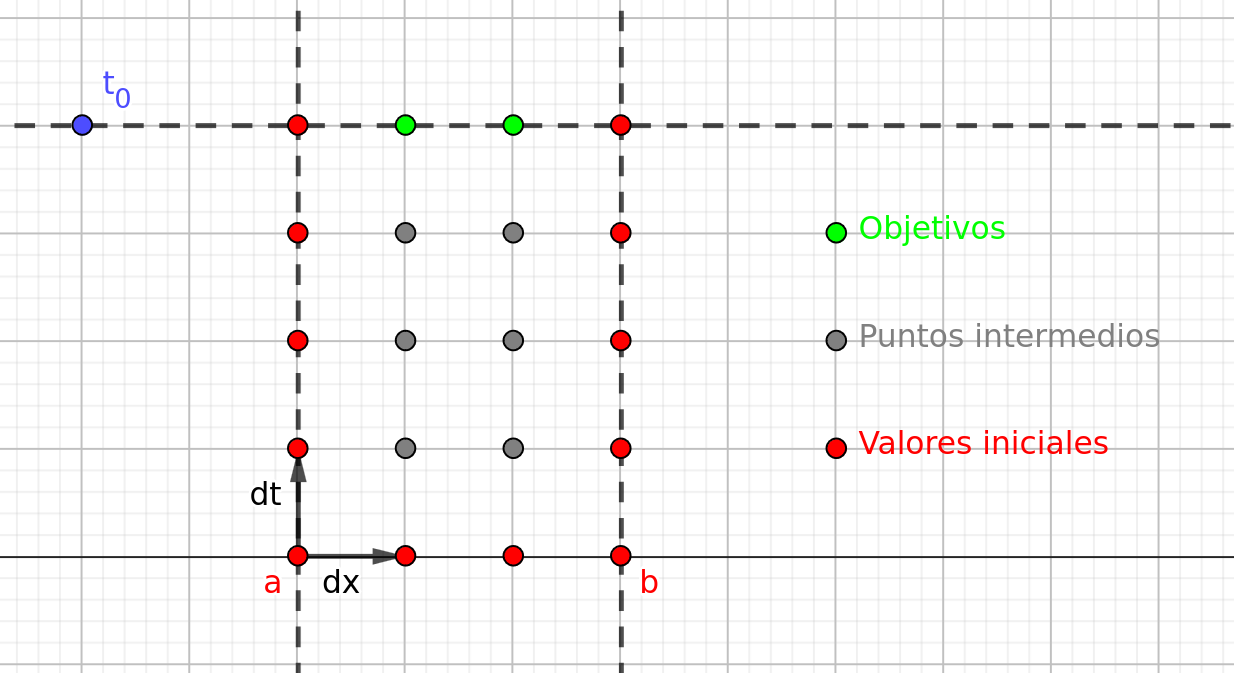
\includegraphics[width=\linewidth]{Imagenes/Bitmap/1dheatpoints.png}
	\caption[Puntos ecuación del calor lineal]{Diagrama que muestra qué puntos intermedios necesitamos calcular para obtener el resultado deseado}
	\label{fig:1dheatpoints}
\end{figure}

Nuestro algoritmo (que puede encontrarse en \ref{code:heat1D_py}) recibe como entrada los siguientes datos:
\begin{itemize}[label=$\bullet$]
	\item \textbf{intervalo}: El intervalo sobre el que vamos a trabajar.
	\item \textbf{$f$, $\alpha$, $\beta$}: Las funciones que determinan las condiciones de contorno.
	\item \textbf{t\_obj}: El tiempo objetivo al que queremos llegar.
	\item \textbf{nt, nx}: El número de fracciones de tiempo (sin incluir la primera) y de fracciones de espacio (sin incluir los extremos) respectivamente.
\end{itemize}

Primero calcula $dt$, $dx$ y $\lambda$ con los datos que le hemos dado, y nos avisa si el método pudiera no converger con esos datos.

Luego rellena la matriz de resultados, comenzando por los valores iniciales (utilizando las funciones $f$, $\alpha$ y $\beta$) y luego va rellenando la tabla con la fórmula de abajo a arriba.


\section{Ecuación del calor en un plano}

\section{Ecuación de onda lineal}
En este caso, la fórmula a implementar es
\begin{equation*}
	u_{i,j+1} =  2\left[1 - \left(c\frac{\Delta t}{\Delta x}\right)^2\right]u_{i,j} + \left(c\frac{\Delta t}{\Delta x}\right)^2[u_{i+1,j} + u_{i-1,j}] - u_{i,j-1}
\end{equation*}
y tenemos unas condiciones iniciales que nos dan el valor de la función en los dos primeros instantes de tiempo para cualquier $x$. Esto hará que para calcular los valores de la solución en el intervalo  $[a,b]$ en $t_0$ necesitaremos conocer bastantes más puntos intermedios que en otros casos, como podemos observar en la figura \ref{fig:1dwavepoints}.

\begin{figure}
	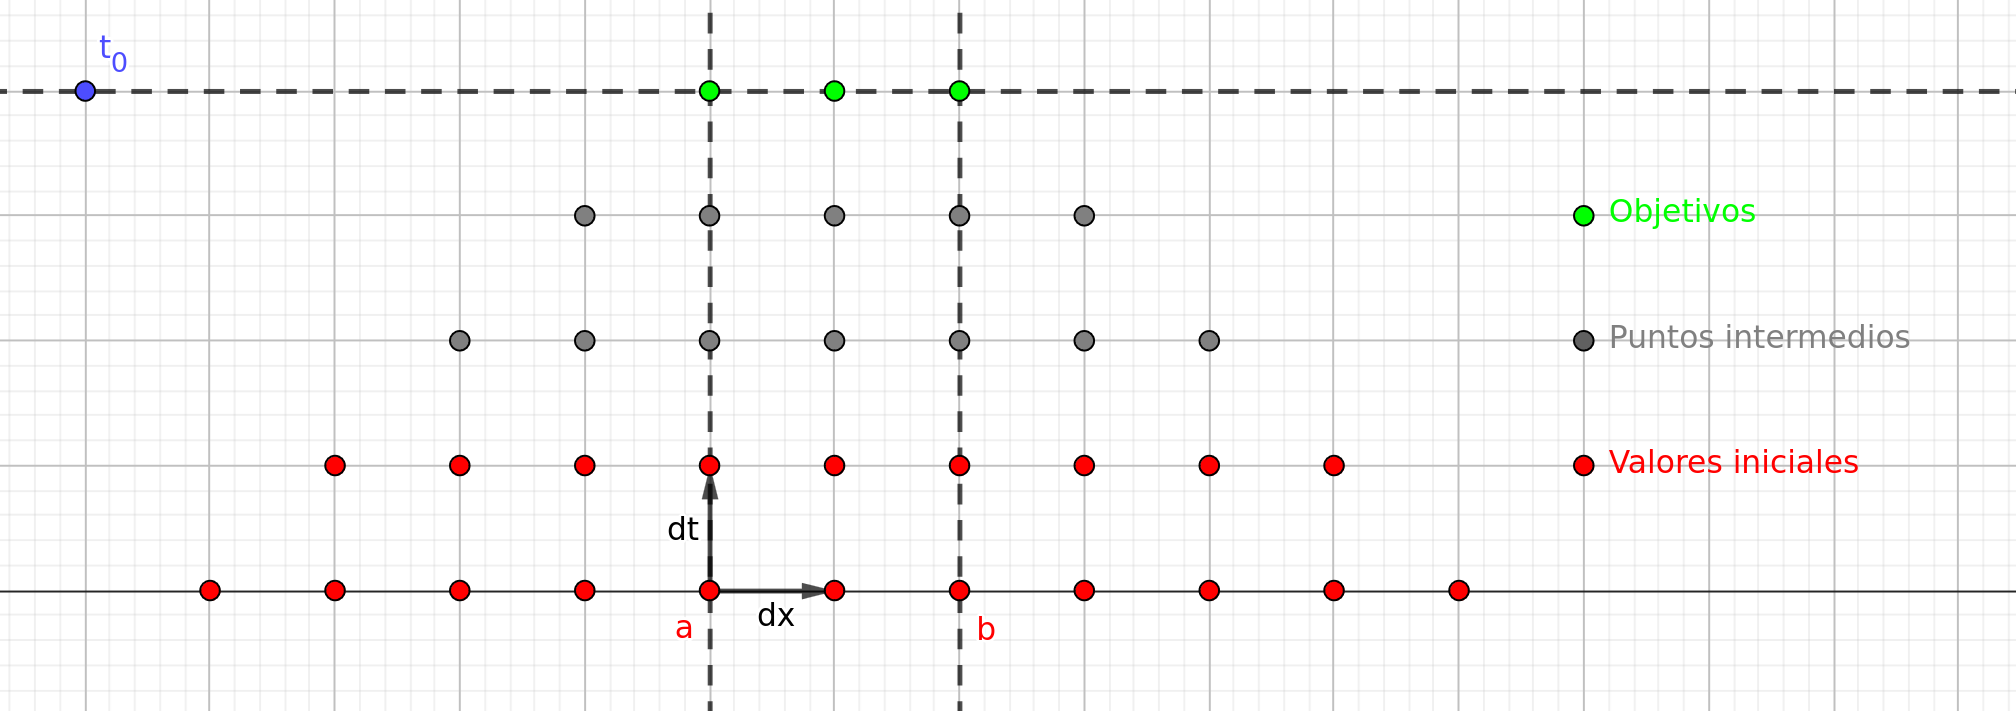
\includegraphics[width=\linewidth]{Imagenes/Bitmap/1dwavepoints.png}
	\caption[Puntos ecuación del calor lineal]{Diagrama que muestra qué puntos intermedios necesitamos calcular para obtener el resultado deseado}
	\label{fig:1dwavepoints}
\end{figure}

El algoritmos (que se encuentra en \ref{code:wave1D_py}), recibe como entrada los siguientes datos:
\begin{itemize}[label=$\bullet$]
	\item \textbf{a, n\_puntos}: El valor inicial del intervalo objetivo y el número de punto que tiene.
	\item \textbf{$f$, $g$, c}: Las funciones que determinan el problema de valor inicial y la constante de la ecuación.
	\item \textbf{t\_obj}: El tiempo objetivo al que queremos llegar.
	\item \textbf{nt}: El número de fracciones de tiempo (sin incluir la primera) que vamos a hacer. El número de fracciones de espacio se calcula a partir de esto para que $\lambda=1$.
\end{itemize}

El algoritmo primero calcula $dt$, $dx$ y $nx$ a partir de los valores que le hemos dado, luego rellena usando las funciones $f$ y $g$ las dos primeras filas de la matriz (valor inicial) y rellena el resto de esta de abajo a arriba utilizando la fórmula.

\section{Ecuación de onda en el plano}

\section{Ecuación de Laplace en el plano}